GENESIS est une soci{\'e}t{\'e} de haute technologie en acoustique bas{\'e}e
dans l'Europ{\^o}le de l'Arbois {\`a} Aix en Provence. Elle est cr{\'e}{\'e}e en
ao{\^u}t 1999 par Patrick Boussard accompagn{\'e} de 6 ing{\'e}nieurs. Son
activit{\'e} se d{\'e}compose en deux parties :\\

\begin{itemize}
   \item la r{\'e}alisation d'{\'e}tudes et d'expertises li{\'e}es {\`a} la simulation
         ou {\`a} la perception des environnements sonores,\\

   \item la conception, la production et la commercialisation de syst{\`e}mes
    audionum{\'e}riques g{\'e}n{\'e}riques ou sp{\'e}cifiques aux besoins des clients.\\
\end{itemize}

\begin{figure}[h]
    \centering
    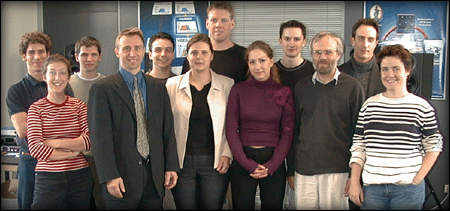
\includegraphics[width=12cm]{figures/equipe.png}\\
    \caption{L'equipe de GENESIS (avec deux stagiaires).}
    \label{equipe}
\end{figure}

GENESIS repose sur une {\'e}quipe de 10 salari{\'e}s. Sa partie recherche,
d{\'e}veloppement et production s'appuie sur des sp{\'e}cialistes dans 4
domaines de comp{\'e}tence :\\

\begin{itemize}
    \item Analyse et synth{\`e}se de son, transformation et traitement du signal
          audionum{\'e}rique.\\

    \item Simulation d'environnement sonore en trois dimensions, spatialisation
          des sources virtuelles.\\

    \item Psychoacoustique - {\'e}tude quantitative et qualitative de la perception
          et de la sensation auditive.\\

    \item Conception et r{\'e}alisation de syst{\`e}mes audionum{\'e}riques, Informatique,
          {\'e}lectronique analogique et num{\'e}rique, industrialisation, production.\\
\end{itemize}

Son savoir-faire est cultiv{\'e} et approfondi par une collaboration
permanente avec des centres de recherches, en particulier avec :\\

\begin{itemize}
    \item L'IRCAM (Institut de Recherche et Coordination Acoustique/Musique)
          {\`a} Paris.\\
    \item Le Laboratoire de M{\'e}canique et d'Acoustique (LMA) du CNRS {\`a} Marseille
          (Equipes Psychoacoustique et Informatique Musicale).\\
\end{itemize}

De plus, elle accueille dans son {\'e}quipe trois {\'e}tudiants effectuant
leur th{\`e}se, ce qui renforce son potentiel en recherche et d{\'e}veloppement.\\

\begin{figure}[h]
    \centering
    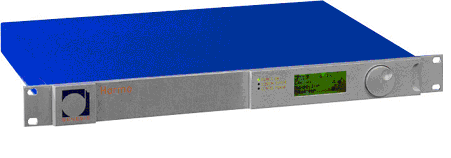
\includegraphics[width=12cm]{figures/harmo.png}\\
    \caption{L'Harmo.}
    \label{harmo}
\end{figure}

Les principales r{\'e}alisations de la soci{\'e}t{\'e} GENESIS sont :\\

\begin{itemize}
    \item l'environnement sonore du simulateur de vol pour les pilotes du
    SuperPuma (client Eurocopter),\\
    \item une {\'e}tude sur les bruits de circulation routi{\`e}re et
    ferroviaire (minist{\`e}re des transports et de l'{\'e}quipement,
    minist{\`e}re de l'environnement),\\
    \item une machine d{\'e}di{\'e}e , l'Harmo (fig. \ref{harmo}),
    permettant l'harmonisation \footnote{changement de
    la dur{\'e}e d'un son en modifiant le moins possible son timbre,
    sa hauteur...} en temps r{\'e}el de bandes sons. GENESIS a re\c{c}u
    le prix de l'innovation technologique Satisfecit pour ce
    produit lors de sa participation au SATIS (octobre 2001).\\
\end{itemize}

Enfin, GENESIS a su gagner la confiance d'importants groupes
industriels pour des {\'e}tudes ou des simulations d'environnements
sonores; on peut citer notamment P.S.A., Michelin, la S.N.C.F.,
Renault...
